\bigbreak
\paragraph*{Ukratko o OpenVPN tehnologiji}
\hfill \smallbreak

OpenVPN\cite{openvpn} besplatan je program za ostvarenje vlastitog virtualnog privatnog tunela preko interneta. OpenVPN-om možemo ostvariti brojna rješenja povezivanja kao što su prijenos podataka, uporaba servera kao pristupne točke na internet, povezivanje udaljenih uređaja u logičku LAN mrežu,...\smallbreak
Neke svojstva OpenVPN povezivanja:
\begin{itemize}
	\item sigurni virtualni tunel na internetu
	\item prijenos podataka TCP ili UDP protokolom
	\item odabir željene vrste šifriranja
	\item višestruko povezivanje
	\item povezivanje računala s različitim operacijskim sustavima
\end{itemize}
\smallbreak
Topologija koja se želi u ovom poglavlju ostvariti jest priključivanje korisnika udaljenoj mreži kao što je ilustrirano na slici \ref{fig:topologija-open}. Korisnik će preko svojeg računala uspostaviti virtualni privatni tunel preko Interneta s računalom koje ima instaliran i konfiguriran OpenVPN server. Nakon povezivanja će korisnik pripadati logičkoj lokalnoj mreži servera.
\begin{figure}[h!]
	\centering
     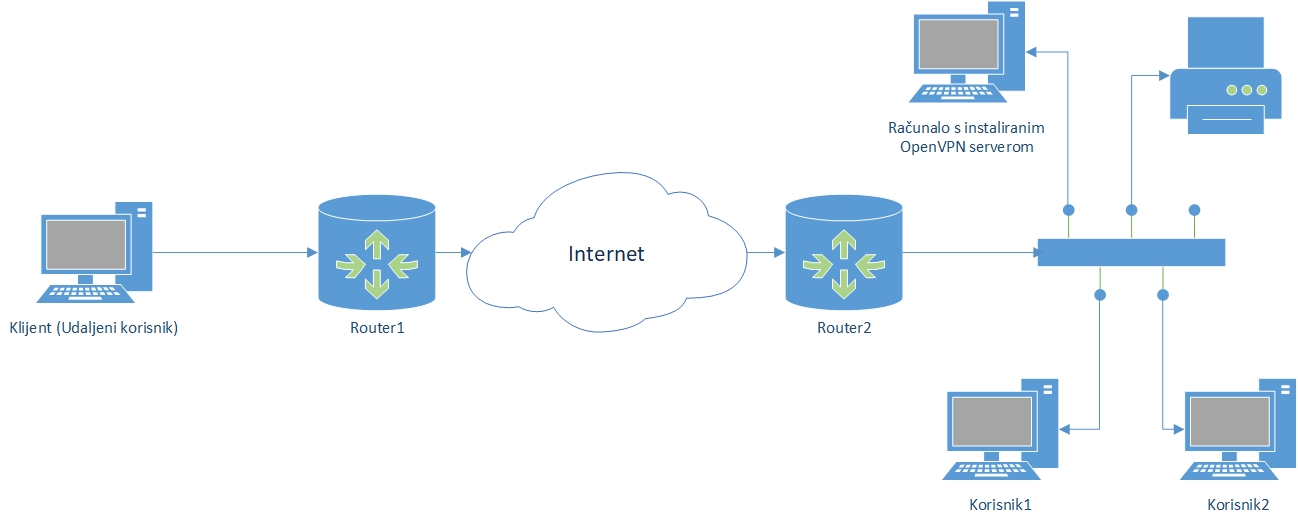
\includegraphics[width=0.9\textwidth]{OVPN-win/topologija}
     \caption{VPN topologija}
     \label{fig:topologija-open}
\end{figure}
\FloatBarrier
\bigbreak
\paragraph*{Instalacija OpenVPN servera}
\hfill \bigbreak
Za početak potrebno je preuzeti instalaciju VPN-a sa službene stranice OpenVPN-a:\\ \url{https://openvpn.net/community-downloads/}
\hfill \smallbreak
Na službenoj stranici potrebno je pokrenuti preuzimanje verzije za operacijski sustav Windows:
\begin{figure}[h!]
	\centering
     
\includegraphics[width=0.8\textwidth]{OVPN-win/slika1}
     \caption{Prikaz poveznice za preuzimanje}
\end{figure}
\FloatBarrier
\begin{wrapfigure}{r}{0.4\textwidth}
  \begin{center}
    
\includegraphics[width=0.2\textwidth]{OVPN-win/slika2}
    \caption{Ikona instalacije}
  \end{center}
\end{wrapfigure}
\FloatBarrier
Ako je uspješno obavljeno preuzimanje, može se započeti instalacija pokretanjem programa s ovakvom ikonom.
\bigbreak
Dalje je potrebno pratiti klasične korake instalacije programa. Kada vam program ponudi odabir direktorija instalacije, preporuka je da odaberete pretpostavljeni direktorij jer su daljnje upute i konfiguracija pravljeni prema tom uzoru. Ako odaberete vlastiti, morate puteve prikazane u daljnjim koracima preoblikovati tako da vode do vašeg direktorija instalacije.
\smallbreak

Obratite pažnju na sljedeću sliku (slika \ref{fig:instalacija-open}) jer prikazuje uz pretpostavljene i važan odabir za uspješnu instalaciju. Potrebno je odabrati i instalirati ``EasyRSA 2 Certificate Management Scripts''.
\begin{figure}[h!]
	\centering
     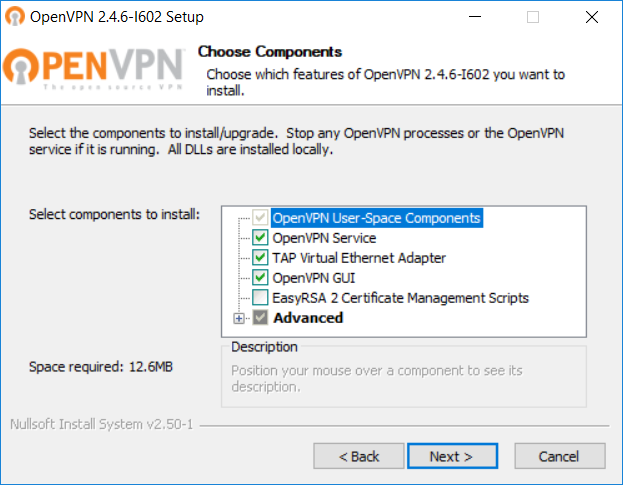
\includegraphics[width=0.7\textwidth]{OVPN-win/slika3}
     \caption{Prikaz dodataka instalacije}
     \label{fig:instalacija-open}
\end{figure}
\FloatBarrier
U sklopu instalacije programa obavljena je i instalacija virtualnog mrežnog priključka na računalu. Taj će se priključak koristiti za povezivanje poslužitelja i klijenata te je vidljiv u postavkama mreže računala:\smallbreak
\small\textcolor{blue}{Upravljačka ploča/Sve stavke upravljačke ploče/Mrežne veze}
\smallbreak
Kako bismo ga lakše adresirali kasnije, promijenit ćemo mu ime u ``ServerVPN''. Adapter se razlikuje od ostalih jer mu je opis ``TAP-Windows Adapter V9''.

\begin{figure}[h!]
    \centering
    \begin{subfigure}[b]{0.35\textwidth}
        
\includegraphics[width=\textwidth]{OVPN-win/slika4}
        \caption{Prije}
        \label{fig:prije}
    \end{subfigure}
    $\Longrightarrow$
    \begin{subfigure}[b]{0.35\textwidth}
        
\includegraphics[width=\textwidth]{OVPN-win/slika5}
        \caption{Nakon}
        \label{fig:nakon}
    \end{subfigure}
    \caption{Preimenovanje TAP adaptera}
\end{figure}
\FloatBarrier

Naredni se koraci izvode upisom naredbi u naredbeni redak. Potrebno je naredbeni redak pokrenuti kao administrator za što je prikazan jedan od mogućih načina na slici \ref{fig:administrator-win}.

\begin{figure}[h!]
	\centering
     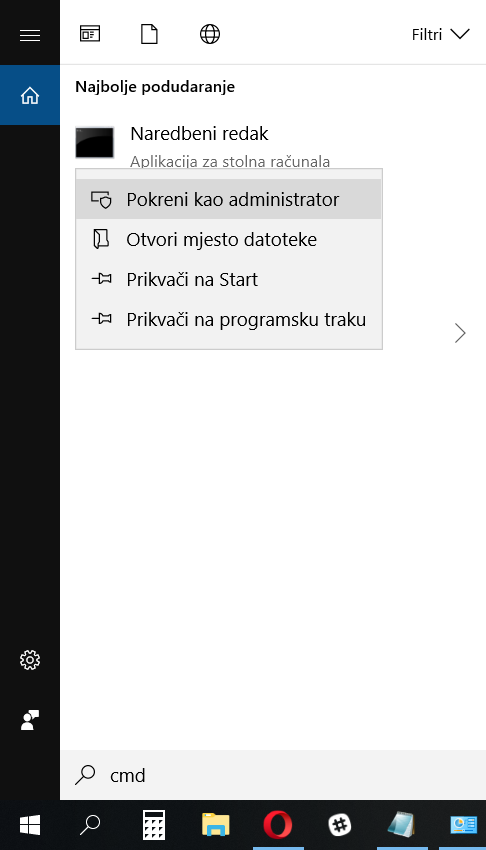
\includegraphics[width=0.4\textwidth]{OVPN-win/slika6}
     \caption{Pokretanje naredbenog retka u administratorskom načinu}
     \label{fig:administrator-win}
\end{figure}
\FloatBarrier

Potrebno se pozicionirati u ``easy-rsa'' direktorij u instalacijskom direktoriju upisom naredbe:
\begin{lstlisting}
cd "C:\Program Files\OpenVPN\easy-rsa"
\end{lstlisting}
Sada je potrebno upisivati po redu sljedeće naredbe.
\begin{lstlisting}
init-config.bat
\end{lstlisting}
Naredba inicijalizira konfiguracijsku datoteku u kojoj možemo dodati informacije o vezi koju uspostavljamo. Ti podaci neće utjecati na rad servera i klijenata.
\begin{lstlisting}
vars
clean-all
build-dh
\end{lstlisting}

\begin{figure}[h!]
	\centering
     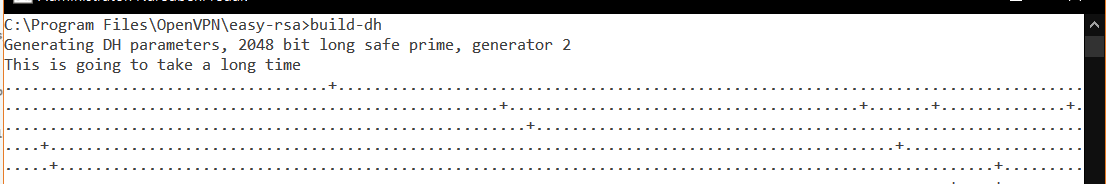
\includegraphics[width=0.9\textwidth]{OVPN-win/slika10}
     \caption{Prikaz pokretanja build-dh naredbe}
\end{figure}
\FloatBarrier
Naredbom se stvara potrebna ``.dh'' datoteka. Na nekim inačicama operacijskog sustava Windows moguća je greška: ``openssl" is not recognized ...\smallbreak
U tom slučaju otići u napredne postavke sustava i dodati ``PATH'' varijablu, tj. put do bin datoteke OpenVPN-a :
\small\textcolor{blue}{C:\textbackslash Program Files\textbackslash OpenVPN\textbackslash bin}
\begin{lstlisting}
build-ca
\end{lstlisting}
Ovom je naredbom započeto stvaranje certifikata potrebnih za sigurno povezivanje servera i klijenata. Prilikom izvršavanja naredbe program nudi polja koja je potrebno popuniti, tj. informacije o našem serveru kako bi se ugradile u ključ što je vidljivo na slici \ref{fig:ca-open}.
\begin{figure}[h!]
	\centering
     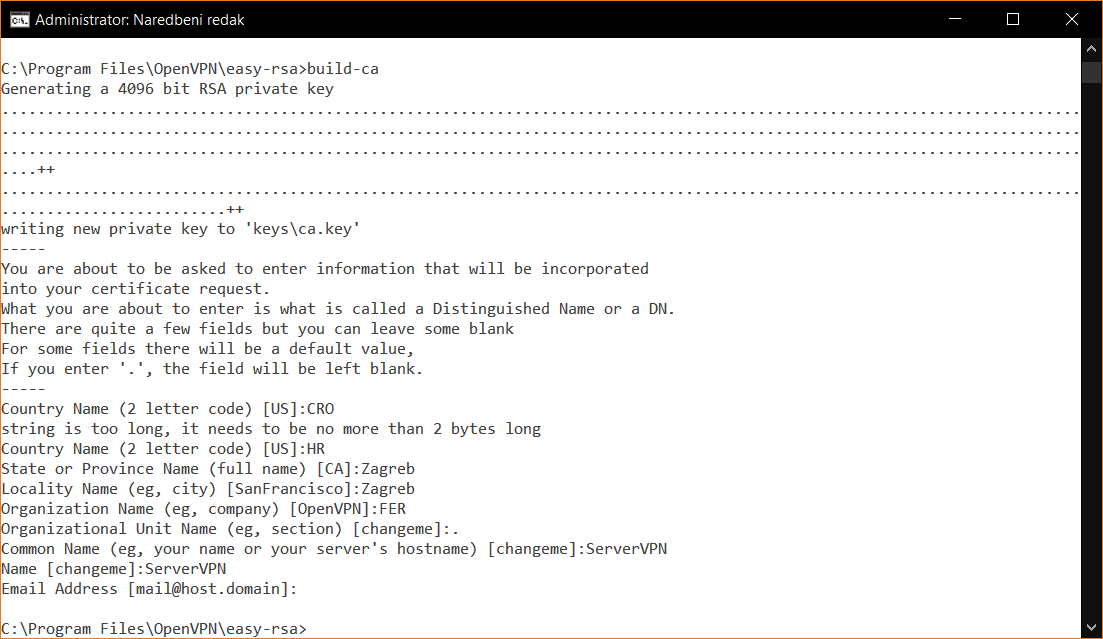
\includegraphics[width=0.9\textwidth]{OVPN-win/slika11}
     \caption{Stvaranje certifikata povezivanja}
     \label{fig:ca-open}
\end{figure}
\FloatBarrier
\begin{lstlisting}
build-key-server ServerVPN
\end{lstlisting}
Ova naredba također nudi upis podataka kao što je vidljivo na slici \ref{fig:serverca-open}, ali ovdje su polja ostavljena prazna jer nisu ključna za rad. Naredbom su nastale 3 datoteke u instalacijskom direktoriju ``.crt'',  ``.csr'' i ``.key''.
\begin{figure}[h!]
	\centering
     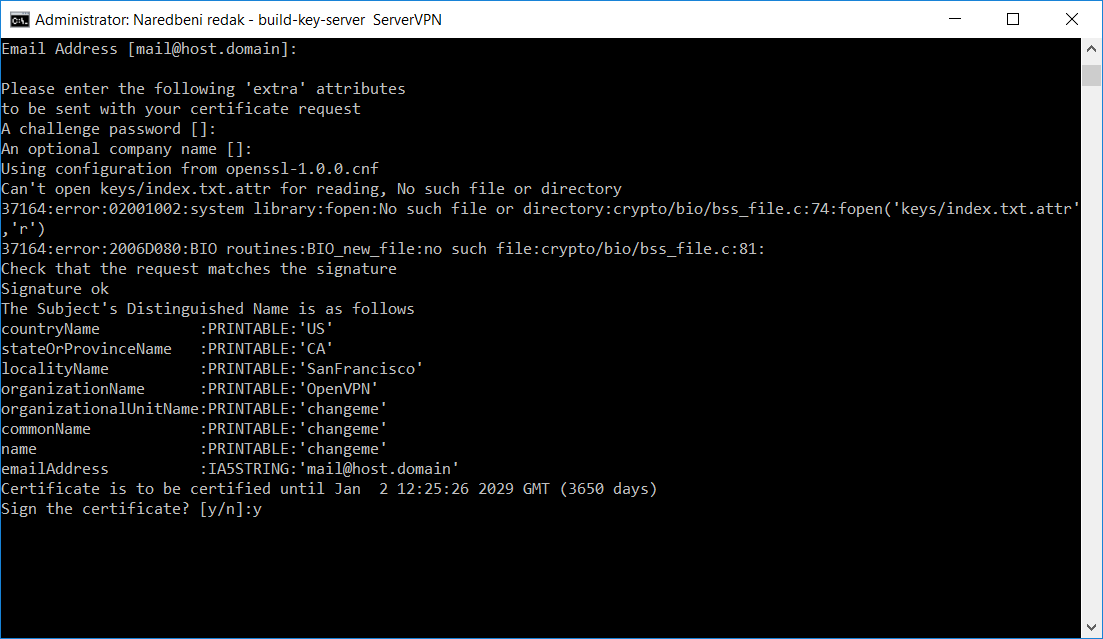
\includegraphics[width=0.9\textwidth]{OVPN-win/slika12}
     \caption{Stvaranje certifikata servera}
     \label{fig:serverca-open}
\end{figure}
\FloatBarrier
Idući korak stvaranje je certifikata klijenta.
\begin{lstlisting}
build-key KlijentVPN
\end{lstlisting}
Po potrebi popuniti podacima o klijentu. Kako bi se razlikovao od ostalih, važno je popuniti polje ``Common Name'' kao na slici \ref{fig:klijent-open} i potvrditi stvaranje.
\begin{figure}[h!]
	\centering
     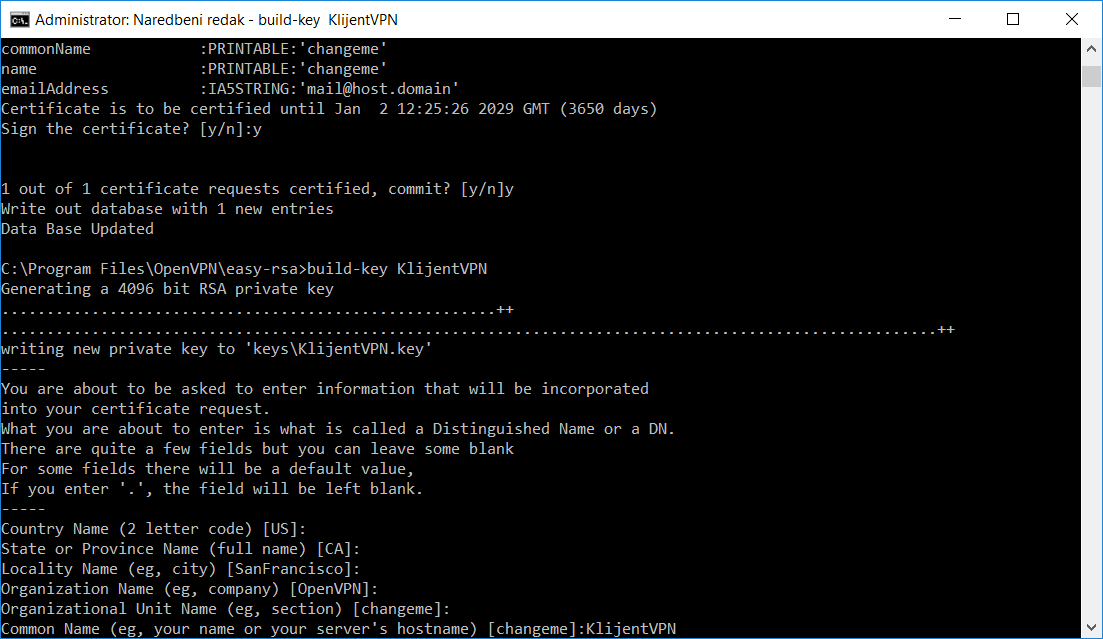
\includegraphics[width=0.9\textwidth]{OVPN-win/slika13}
     \caption{Stvaranje certifikata klijenta}
     \label{fig:klijent-open}
\end{figure}
\FloatBarrier
Kao i u prethodnom koraku nastale su 3 datoteke. Sve su neophodne za prijavu na naš server zato ih mi moramo spremiti i prebaciti na računala koja će se htjeti povezati na server. Povezivanje na server objašnjeno je u jednom od sljedećih dijelova poglavlja.\smallbreak
Moguće je naravno dodavanje više različitih korisnika i brisanje istih.
\begin{lstlisting}
openvpn --genkey --secret keys/ta.key
\end{lstlisting}

Ovom naredbom stvara se ključ kojim se autentificiraju podaci između servera i klijenata.
 
\paragraph*{Konfiguracija OpenVPN servera}
\hfill \bigbreak
Konfiguracijske datoteke ne postoje same po sebi pa ih je potrebno stvoriti na radnoj površini kao prazan tekstualni dokument, spremiti u obliku ``ServerVPN.ovpn'' datoteke pa kopirati u direktorij OpenVPN-a na lokaciju:\smallbreak
\small\textcolor{blue}{C:\textbackslash Program Files\textbackslash OpenVPN\textbackslash config}
\smallbreak

``Server.ovpn'' jest konfiguracijska datoteka stvorenog servera. OpenVPN nudi brojne postavke koje serveru daju širok izbor svojstava i mogućnosti. Naglasak ovih uputa je na povezivanju klijenata i servera te su dodane mogućnosti samo s tim ciljem.\smallbreak
Konfiguracijska datoteka treba sadržavati:\smallbreak
{\small\fontfamily{pcr}\selectfont
dev-node "ServerVPN"\hfill;ime

mode server\hfill;uloga u mreži

port 12345\hfill;vrata preko kojih ide komunikacija	

proto tcp4-server\hfill;protokol prijenosa

dev tun\hfill;stvara se virtualni tunel

tls-server\hfill;za autentifikaciju

tls-auth "C:\textbackslash \textbackslash Program Files\textbackslash \textbackslash OpenVPN\textbackslash \textbackslash easy-rsa\textbackslash \textbackslash keys\textbackslash \textbackslash ta.key" 0\hfill

; put do datoteke ključa(ta.key) te broj 0 koja označava server

tun-mtu 1500\hfill;veličina MTU paketa

tun-mtu-extra 32\hfill;veličina MTU paketa

mssfix 1450\hfill;veličina MTU paketa

ca "C:\textbackslash \textbackslash Program Files\textbackslash \textbackslash OpenVPN\textbackslash \textbackslash easy-rsa\textbackslash \textbackslash keys\textbackslash \textbackslash ca.crt"\hfill

; put do datoteke ca.crt

cert "C:\textbackslash \textbackslash Program Files\textbackslash \textbackslash OpenVPN\textbackslash \textbackslash easy-rsa\textbackslash \textbackslash keys\textbackslash \textbackslash ServerVPN.crt"\hfill

; put do certifikata servera

key "C:\textbackslash \textbackslash Program Files\textbackslash \textbackslash OpenVPN\textbackslash \textbackslash easy-rsa\textbackslash \textbackslash keys\textbackslash \textbackslash ServerVPN.key"\hfill

; put do ključa servera

dh "C:\textbackslash \textbackslash Program Files\textbackslash \textbackslash OpenVPN\textbackslash \textbackslash easy-rsa\textbackslash \textbackslash keys\textbackslash \textbackslash dh2048.pem"\hfill

; put do .dh datoteke

server 10.10.10.0 255.255.255.0\hfill

; virtualna adresa servera i maska podmreže

client-to-client\hfill; klijenti se vide

keepalive 10 120\hfill; vrijeme čekanja na vezu

cipher AES-128-CBC\hfill; vrsta šifriranja

comp-lzo\hfill; kompresija podataka u tunelu

persist-key\hfill;za slučaj prekida veze

persist-tun\hfill;za slučaj prekida veze

client-config-dir "C:\textbackslash \textbackslash Program Files\textbackslash \textbackslash OpenVPN\textbackslash \textbackslash config"\hfill

;direktorij konfiguracije

verb 3\hfill;stupanj ispisa grešaka i upozorenja

route-delay 5\hfill;čekanje do početka primanja zahtjeva

route-method exe\hfill;način unosa rute

push "route 161.53.63.0 255.255.255.0" 

route 161.53.63.204 255.255.255.0\hfill

;adresa koju je router dodijelio računalu na kojem uspostavljamo server
}\bigbreak
Za upute i pojašnjenja kako odabrati ispravne vlastite parametre za ovu datoteku molimo pogledajte detaljnije upute na adresi:\smallbreak \url{https://openvpn.net/community-resources/how-to/\#config}\smallbreak
Osim toga potrebno je:
\begin{itemize}
	\item imati stabilnu vezu na internet i statičku IP adresu
	\item imati omogućenu razmjenu TCP paketa u firewallu
	\item imati omogućeno prosljeđivanje prometa s routera na vrata na kojima server sluša (Port forwarding)
\end{itemize}	
	
Ako je konfiguracija dobro odrađena moguće je pokrenuti server. Povezivanje se započinje pokretanjem ``OpenVPN GUI'' datoteke na radnoj površini, odabirom ikone računala s alatne trake i odabirom ``Connect'' mogućnosti što je prikazano na slici \ref{fig:povezivanje-open}. 
\begin{figure}[h!]
	\centering
     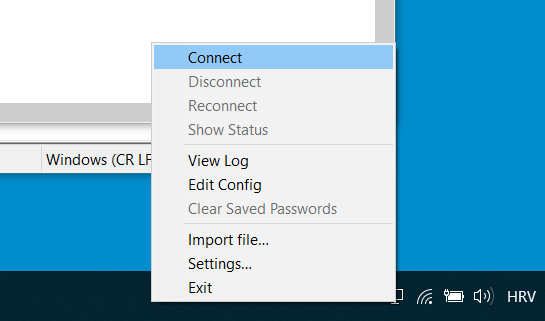
\includegraphics[width=0.5\textwidth]{OVPN-win/slika15}
     \caption{Povezivanje sa serverom}
     \label{fig:povezivanje-open}
\end{figure}
\FloatBarrier 	
Pokrenut bi server trebao izgledati kao na slici \ref{fig:status-open}.
\begin{figure}[h!]
	\centering
     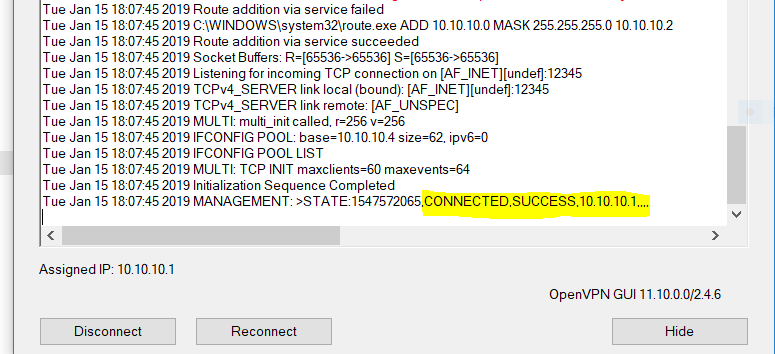
\includegraphics[width=0.7\textwidth]{OVPN-win/slika16}
     \caption{Status servera}
     \label{fig:status-open}
\end{figure}
\FloatBarrier
\newpage
\paragraph*{Konfiguracija OpenVPN klijenta}
\hfill \bigbreak

Kao prvi korak potrebno je instalirati OpenVPN kao i za server sa adrese:\smallbreak

\url{https://openvpn.net/community-downloads/}\smallbreak

Prilikom instalacije nije potrebno odabrati dodatne mogućnosti.\smallbreak
Na klijentskom računalu stvorite datoteku ``Klijent.ovpn" i kopirajte ju u 

\small\textcolor{blue}{C:\textbackslash Program Files\textbackslash OpenVPN\textbackslash easy-rsa\textbackslash keys}

\begin{figure}[h!]
	\centering
     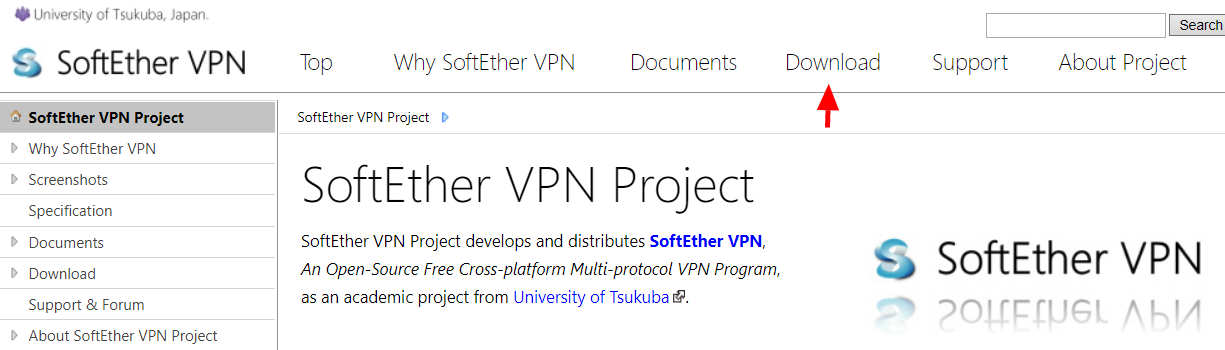
\includegraphics[width=0.2\textwidth]{OVPN-win/korak1}
     \caption{Prikaz Klijent.ovpn datoteke}
\end{figure}
\FloatBarrier

Konfiguracijska datoteka treba sadržavati:\smallbreak
{\small\fontfamily{pcr}\selectfont
remote 161.53.63.204\hfill;javna IP adresa računala sa serverom

client\hfill;ime uloge u mreži

port 12345\hfill;broj vrata veze

proto tcp4-client\hfill;protokol prijenosa

dev tun\hfill;stvara se virtualni tunel

tls-client\hfill;za autentifikaciju

tls-auth "C:\textbackslash \textbackslash Program Files\textbackslash \textbackslash OpenVPN\textbackslash \textbackslash easy-rsa\textbackslash \textbackslash keys\textbackslash \textbackslash ta.key" 1\hfill

; put do datoteke ključa(ta.key) te broj 1 koja označava klijenta

remote-cert-tls server

tun-mtu 1500\hfill;veličina MTU paketa

tun-mtu-extra 32\hfill;veličina MTU paketa

mssfix 1450\hfill;veličina MTU paketa

ca "C:\textbackslash \textbackslash Program Files\textbackslash \textbackslash OpenVPN\textbackslash \textbackslash easy-rsa\textbackslash \textbackslash keys\textbackslash \textbackslash ca.crt"\hfill

; put do datoteke ca.crt

cert "C:\textbackslash \textbackslash Program Files\textbackslash \textbackslash OpenVPN\textbackslash \textbackslash easy-rsa\textbackslash \textbackslash keys\textbackslash \textbackslash KlijentVPN.crt"\hfill

; put do certifikata klijenta

key "C:\textbackslash \textbackslash Program Files\textbackslash \textbackslash OpenVPN\textbackslash \textbackslash easy-rsa\textbackslash \textbackslash keys\textbackslash \textbackslash KlijentVPN.key"\hfill

; put do ključa klijenta

cipher AES-128-CBC\hfill; vrsta šifriranja

comp-lzo\hfill; kompresija podataka u tunelu

persist-key\hfill;za slučaj prekida veze

persist-tun\hfill;za slučaj prekida veze

verb 3\hfill;stupanj ispisa grešaka i upozorenja

}\bigbreak

Za upute i pojašnjenja kako odabrati ispravne vlastite parametre za ovu datoteku molimo pogledajte detaljnije upute na adresi:\smallbreak \url{https://openvpn.net/community-resources/how-to/\#config}\smallbreak

Osim toga potrebno je:
\begin{itemize}
	\item imati stabilnu vezu na internet
	\item imati omogućenu razmjenu TCP paketa u firewallu
\end{itemize}	

\paragraph*{Povezivanje klijenta i servera}
\hfill \bigbreak
Kako bi se klijent uspješno povezao na server, iz instalacijskog direktorija SERVERA kopirajte sljedeće datoteke u novu mapu koju ćete prebaciti na računala klijenata:\smallbreak
{\small\fontfamily{pcr}\selectfont
ta.key

KlijentVPN.key

KlijentVPN.csr

KlijentVPN.crt

ca.crt
}\smallbreak
Prebaciti željenim načinom na klijentsko računalo ili računala koja će se povezivati na server i kopirati u instalacijski direktorij na adresi:\smallbreak
\small\textcolor{blue}{C:\textbackslash Program Files\textbackslash OpenVPN\textbackslash easy-rsa\textbackslash keys}
\smallbreak
Ako je konfiguracija dobro odrađena, moguće je povezivanje na server. Povezivanje se započinje pokretanjem ``OpenVPN GUI'' datoteke na radnoj površini, odabirom ikone računala s alatne trake i odabirom ``Connect'' mogućnosti.
\bigbreak
Na nekim verzijama operacijskih sustava Windows potrebno je dodatno omogućiti povezivanje na interne adrese servera(npr. kao što smo postavili na 10.10.10.5) na sljedeći način:
\begin{enumerate}
  \item U tražilicu računala upisati \small\textcolor{blue}{regedit}
  \item Pozicionirati se na lokaciju s adresom \small\textcolor{blue}{Computer\textbackslash HKEY\_LOCAL\_MACHINE\newline
  \textbackslash SYSTEM\textbackslash CurrentControlSet\textbackslash Services\textbackslash Tcpip\textbackslash Parameters}
  \item Pronaći IPEnableRouter te postaviti vrijednost na 1 i na računalu servera i na računalu klijenta
\end{enumerate}
\bigbreak

Prilikom komplikacija ili nejasnoća pogledati detaljnije upute na adresi:\smallbreak
\url{https://openvpn.net/community-resources/how-to/\#config}
\smallbreak